% This file was created with tikzplotlib v0.9.14.
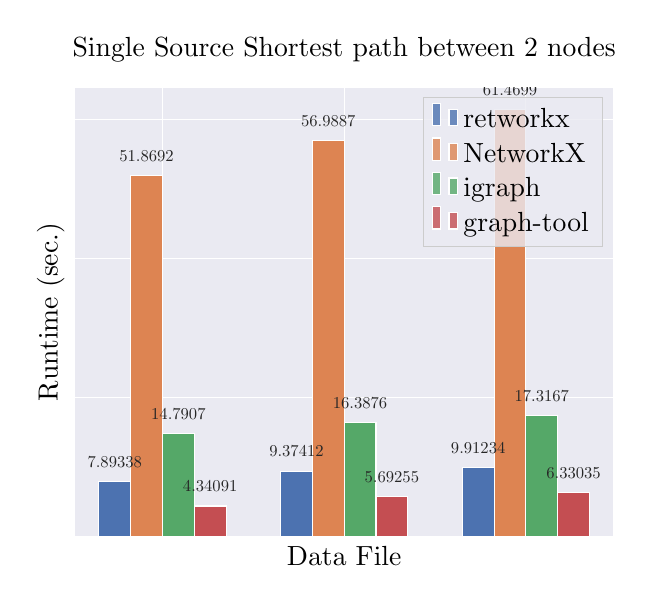
\begin{tikzpicture}

\definecolor{color0}{rgb}{0.917647058823529,0.917647058823529,0.949019607843137}
\definecolor{color1}{rgb}{0.298039215686275,0.447058823529412,0.690196078431373}
\definecolor{color2}{rgb}{0.866666666666667,0.517647058823529,0.32156862745098}
\definecolor{color3}{rgb}{0.333333333333333,0.658823529411765,0.407843137254902}
\definecolor{color4}{rgb}{0.768627450980392,0.305882352941176,0.32156862745098}

\begin{axis}[
axis background/.style={fill=color0},
axis line style={white},
legend cell align={left},
legend style={fill opacity=0.8, draw opacity=1, text opacity=1, draw=white!80!black, fill=color0},
tick align=outside,
title={Single Source Shortest path between 2 nodes},
x grid style={white},
xlabel={Data File},
xmajorgrids,
xmajorticks=false,
xmin=-0.485, xmax=2.485,
xtick style={color=white!15!black},
xtick={0,1,2},
xticklabels={USA-road-1.USA,USA-road-d.USA,USA-road-t.USA},
y grid style={white},
ylabel={Runtime (sec.)},
ymajorgrids,
ymajorticks=false,
ymin=0, ymax=64.5433534812927,
ytick style={color=white!15!black}
]
\draw[draw=white,fill=color1] (axis cs:-0.35,0) rectangle (axis cs:-0.175,7.89337859153748);
\addlegendimage{ybar,ybar legend,draw=white,fill=color1}
\addlegendentry{retworkx}

\draw[draw=white,fill=color1] (axis cs:0.65,0) rectangle (axis cs:0.825,9.37411952018738);
\draw[draw=white,fill=color1] (axis cs:1.65,0) rectangle (axis cs:1.825,9.91233687400818);
\draw[draw=white,fill=color2] (axis cs:-0.175,0) rectangle (axis cs:0,51.8691621303558);
\addlegendimage{ybar,ybar legend,draw=white,fill=color2}
\addlegendentry{NetworkX}

\draw[draw=white,fill=color2] (axis cs:0.825,0) rectangle (axis cs:1,56.9886650085449);
\draw[draw=white,fill=color2] (axis cs:1.825,0) rectangle (axis cs:2,61.469860458374);
\draw[draw=white,fill=color3] (axis cs:1.38777878078145e-17,0) rectangle (axis cs:0.175,14.7906747817993);
\addlegendimage{ybar,ybar legend,draw=white,fill=color3}
\addlegendentry{igraph}

\draw[draw=white,fill=color3] (axis cs:1,0) rectangle (axis cs:1.175,16.3875679969788);
\draw[draw=white,fill=color3] (axis cs:2,0) rectangle (axis cs:2.175,17.3167360305786);
\draw[draw=white,fill=color4] (axis cs:0.175,0) rectangle (axis cs:0.35,4.34091234207153);
\addlegendimage{ybar,ybar legend,draw=white,fill=color4}
\addlegendentry{graph-tool}

\draw[draw=white,fill=color4] (axis cs:1.175,0) rectangle (axis cs:1.35,5.692547082901);
\draw[draw=white,fill=color4] (axis cs:2.175,0) rectangle (axis cs:2.35,6.33034567832947);
\draw (axis cs:-0.2625,7.89337859153748) ++(0pt,3pt) node[
  scale=0.6,
  anchor=south,
  text=white!15!black,
  rotate=0.0
]{7.89338};
\draw (axis cs:0.7375,9.37411952018738) ++(0pt,3pt) node[
  scale=0.6,
  anchor=south,
  text=white!15!black,
  rotate=0.0
]{9.37412};
\draw (axis cs:1.7375,9.91233687400818) ++(0pt,3pt) node[
  scale=0.6,
  anchor=south,
  text=white!15!black,
  rotate=0.0
]{9.91234};
\draw (axis cs:-0.0875,51.8691621303558) ++(0pt,3pt) node[
  scale=0.6,
  anchor=south,
  text=white!15!black,
  rotate=0.0
]{51.8692};
\draw (axis cs:0.9125,56.9886650085449) ++(0pt,3pt) node[
  scale=0.6,
  anchor=south,
  text=white!15!black,
  rotate=0.0
]{56.9887};
\draw (axis cs:1.9125,61.469860458374) ++(0pt,3pt) node[
  scale=0.6,
  anchor=south,
  text=white!15!black,
  rotate=0.0
]{61.4699};
\draw (axis cs:0.0875,14.7906747817993) ++(0pt,3pt) node[
  scale=0.6,
  anchor=south,
  text=white!15!black,
  rotate=0.0
]{14.7907};
\draw (axis cs:1.0875,16.3875679969788) ++(0pt,3pt) node[
  scale=0.6,
  anchor=south,
  text=white!15!black,
  rotate=0.0
]{16.3876};
\draw (axis cs:2.0875,17.3167360305786) ++(0pt,3pt) node[
  scale=0.6,
  anchor=south,
  text=white!15!black,
  rotate=0.0
]{17.3167};
\draw (axis cs:0.2625,4.34091234207153) ++(0pt,3pt) node[
  scale=0.6,
  anchor=south,
  text=white!15!black,
  rotate=0.0
]{4.34091};
\draw (axis cs:1.2625,5.692547082901) ++(0pt,3pt) node[
  scale=0.6,
  anchor=south,
  text=white!15!black,
  rotate=0.0
]{5.69255};
\draw (axis cs:2.2625,6.33034567832947) ++(0pt,3pt) node[
  scale=0.6,
  anchor=south,
  text=white!15!black,
  rotate=0.0
]{6.33035};
\end{axis}

\end{tikzpicture}
